\section{Parametrisierte Kurven}
Vier robotergesteuerte Fahrzeuge bewegen sich auf einer ebenen Fläche. Zur Lokalisierung der Fahrzeuge wurde ein kartesisches Koordinatensystem auf die Fläche gezeichnet. Die Position der Fahrzeuge \(F_1, F_2, F_3\) und \(F_4\) zur Zeit \(t\) wird durch die folgenden Gleichungen bestimmt:

\[
    F_1 : \begin{pmatrix}
        x \\y
    \end{pmatrix}
    =
    \begin{pmatrix}
        -8 + 4t \\
        2t
    \end{pmatrix}
    \quad
    F_2 : \begin{pmatrix}
        x \\y
    \end{pmatrix}
    = \begin{pmatrix}
        10 - 2t \\
        -6 + t
    \end{pmatrix}
    \quad
    F_3 : \begin{pmatrix}
        x \\y
    \end{pmatrix}
    =
    \begin{pmatrix}
        2 \cos\left(\frac{\pi}{4}t\right) \\
        2 \sin\left(\frac{\pi}{4}t\right)
    \end{pmatrix}
    \quad
    F_4 : \begin{pmatrix}
        x \\y
    \end{pmatrix}
    = \begin{pmatrix}
        t \\
        \frac{t^2}{4}
    \end{pmatrix}
\]

Diese Gleichungen müssen so interpretiert werden: Das Fahrzeug \(F_1\) befindet sich zur Zeit \(t=2\) im Punkt mit den Koordinaten \(x = -8 + 4 \cdot 2\) und \(y = 2 \cdot 2\).

Skizzieren Sie die Bahn der vier Fahrzeuge in das Koordinatensystem unten.

Kommt es zur Kollision zwischen zwei Fahrzeugen?
\begin{center}
    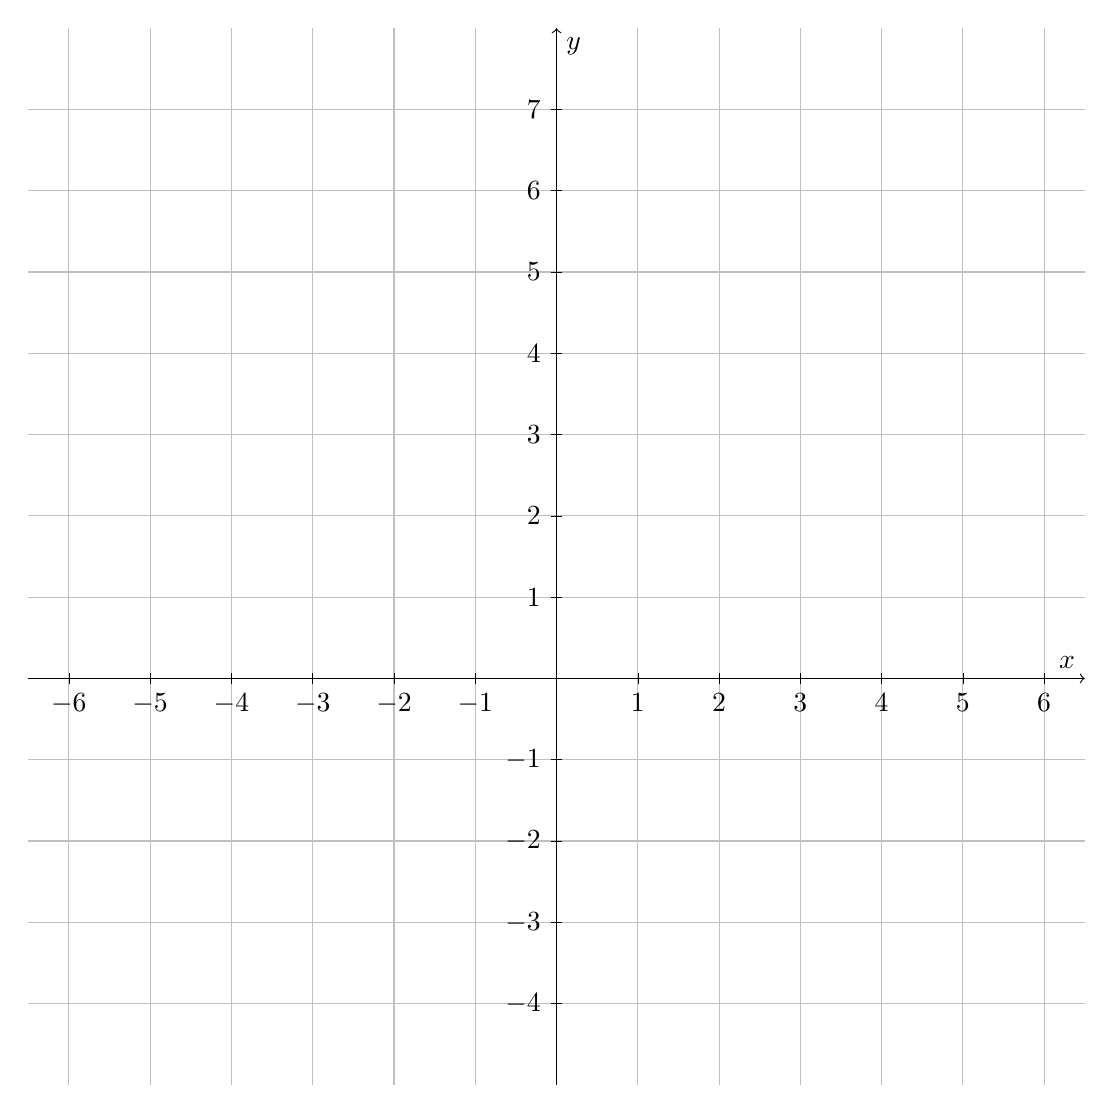
\begin{tikzpicture}
        \begin{axis}[
                grid=both,
                xmin=-6.5, xmax=6.5,
                ymin=-4.5, ymax=7.5,
                axis lines=middle,
                xlabel={\(x\)},
                ylabel={\(y\)},
                xtick={-6, -5, ..., 6},
                ytick={-4, -3, ..., 7},
                width=15cm, height=15cm,
                enlargelimits=false,
                axis equal,
                axis line style={->},
                tick style={color=black}
            ]
        \end{axis}
    \end{tikzpicture}
\end{center}

\clearpage

\begin{definition}
    {Parametrisierte Kurven}{}
    Eine \emph{Parametergleichung einer ebenen Kurve} ist eine Funktion der Form
    \[
        \vec{r}: \mathbb{R} \to \mathbb{R}^2, \quad t \mapsto \vec{r}(t) = \begin{pmatrix}
            x(t) \\
            y(t)
        \end{pmatrix}
    \]
    Dabei ist \( \vec{r}(t) \) der Ortsvektor des Bildpunktes von \( t \in \mathbb{R} \). Die Menge aller Bildpunkte bildet eine Kurve in der Ebene \( \mathbb{R}^2 \).

    Wenn man \( \vec{r}(t) \) als den Ortsvektor eines bewegten Objektes zur Zeit \( t \) auffasst, spricht man auch von einer \emph{ebenen Ortsfunktion}. Die Menge aller Bildpunkte heisst dann \emph{Bahn}.

\end{definition}
\begin{bsp}{}{paramKurveVsGraph}
    Die Ebene Kurve mit der Parametergleichung \( \vec{r}(t) = \begin{pmatrix}
        2\cos(4t) \\ 2 \sin(t)
    \end{pmatrix}\) sieht wie folgt aus:
    \begin{center}
        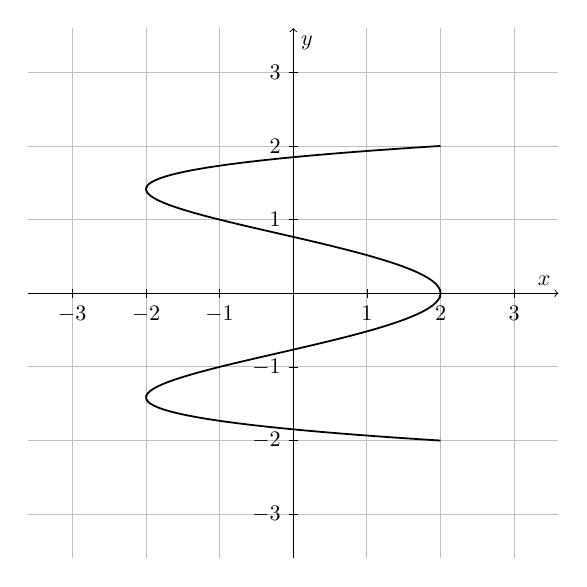
\begin{tikzpicture}[scale=0.8]
            \begin{axis}[
                    axis equal,
                    grid=both,
                    xmin=-3, xmax=3,
                    ymin=-3, ymax=3,
                    axis lines=middle,
                    xlabel={\(x\)},
                    ylabel={\(y\)},
                    xtick={-3, -2, -1, 0, 1, 2, 3},
                    ytick={-3, -2, -1, 0, 1, 2, 3},
                    width=10cm, height=10cm,
                    enlargelimits=true,
                    axis line style={->},
                    tick style={color=black}
                ]
                \addplot[domain=0:2*pi, samples=200, smooth, thick]
                ({2*cos(4*deg(x))}, {2*sin(deg(x))});
            \end{axis}
        \end{tikzpicture}
    \end{center}

\end{bsp}
Dieses Beispiel verdeutlicht, dass parametrisierte Kurven nicht immer Graphen einer Funktion sind.
Umgekehrt kann aber jeder Graph einer Funktion als parametrisierte Kurve aufgefasst werden: Der Graph einer Funktion \( f: \mathbb{R} \to \mathbb{R} \) entspricht der Kurve mit der Parametergleichung
\[
    k: \quad \begin{pmatrix}
        x \\y
    \end{pmatrix} = \begin{pmatrix}
        t \\
        f(t)
    \end{pmatrix}
\]
In gewissen Fällen können die Parametergleichungen in Koordinatengleichungen umgeformt werden. Betrachten Sie dazu die folgenden Beispiele:
\begin{bsp}{Geraden}{}
    Die Darstellung von Geraden wie jener aus der Einführungsfrage mit der Parametergleichung
    \(g: \, \begin{pmatrix}
        x \\y
    \end{pmatrix}
    = \begin{pmatrix}
        10 - 2t \\
        -6 + t
    \end{pmatrix}\) kennen Sie vielleicht schon aus dem im Grundlagenfach. In der Vektorgeometrie werden Geraden häufig so dargestellt:
    \[g: \,\begin{pmatrix}
            x \\y
        \end{pmatrix}
        = \begin{pmatrix}
            10 \\
            -6
        \end{pmatrix}
        + t \cdot\begin{pmatrix}
            -2 \\1
        \end{pmatrix}
    \]
    Aus dieser Parametergleichung kann man leicht die Koordinatengleichung der Geraden ermitteln. Dazu muss man  die Variable \( t \) aus dem obigen Gleichungssystem eliminieren. In diesem Fall könnte man die untere Gleichung nach \( t \) auflösen:
    \[
        t = y + 6
    \]
    Dies kann man in die obere Gleichung einsetzen:
    \[
        x = 10 - 2(y + 6)
    \]
    Das ist schon eine Koordinatengleichung der Geraden \( g \). Wenn man sie nach \( y \) auflöst, erhält man die bekannte Form:
    \[
        g: \quad y = -\frac{1}{2} x - 1.
    \]


\end{bsp}
\begin{bsp}{Kreise}{}
    Die Kurve  mit der Parametergleichung
    \[ k: \, \begin{pmatrix}
            x \\ y
        \end{pmatrix} =
        \begin{pmatrix}
            \cos\left(t\right) \\
            \sin\left(t\right)
        \end{pmatrix}
    \]
    beschreibt einen Kreis mit Radius 1.

    Auch in diesem Beispiel lässt sich eine Koordinatengleichung für den Kreis herleiten, wenn man den Parameter \(t\) im Gleichungssystem eliminiert:
    Wenn man die erste Gleichung nach \( t \) auflöst, erhält man
    \[
        t = \arccos x
    \]
    In die zweite Gleichung eingesetzt, liefert das
    \[
        y = \sin(\arccos(x)).
    \]
    Das ist zwar schon eine Koordinatengleichung, aber man erkennt den Kreis darin nicht. Einfacher wird es, wenn man das Resultat noch bearbeitet. Zu diesem Zweck verwenden wir den trigonometrischen Pythagoras: \( (\sin \alpha)^2 + (\cos \alpha)^2 = 1 \) oder \( \sin \alpha = \pm \sqrt{1 - (\cos \alpha)^2} \). Daraus folgt
    \[
        \begin{aligned}
            y & = \sin(\arccos(x))                    \\
              & = \pm \sqrt{1 - (\cos(\arccos(x)))^2} \\
              & = \pm \sqrt{1 - x^2}
        \end{aligned}
    \]
    Durch Quadrieren und Umordnen erhält man schließlich die bekannte Kreisgleichung
    \[
        x^2 + y^2 = 1
    \]

    Variante

    Mit der richtigen Idee geht das Ganze viel schneller: Man summiert das Quadrat der ersten Gleichung und jenes der zweiten. Dann wird der Parameter \( t \) aus der Gleichung eliminiert und man erhält direkt
    \[
        x^2 + y^2 = (\cos t)^2 + (\sin t)^2 = 1
    \]

\end{bsp}

In Geogebra lassen sich parametrisierte Kurven darstellen. Dazu verwendet man den Befehl Kurve(x, y, t, a, b). Die Kurve aus \Cref*{bsp:paramKurveVsGraph} kann mit folgender Eingabe in Geogebra dargestellt werden: Kurve (2 cos(4 t), 2 sin(t), t, 0, 2*pi)

\begin{ueb}{}{}
    Durch die folgenden Parameterdarstellungen werden Kurven beschrieben. Zeichnen Sie diese Kurven und geben Sie nach Möglichkeit die Kurvengleichung in kartesischer Form an. Überprüfen Sie das Resultat mit Geogebra
    \begin{enumerate}
        \item \(\begin{pmatrix}
                  x \\
                  y
              \end{pmatrix} = \begin{pmatrix}
                  t - 1 \\
                  2t
              \end{pmatrix}\)
        \item \(\begin{pmatrix}
                  x \\
                  y
              \end{pmatrix} = \begin{pmatrix}
                  1 \\
                  t
              \end{pmatrix}\)
        \item \(\begin{pmatrix}
                  x \\
                  y
              \end{pmatrix} = \begin{pmatrix}
                  t - 2 \\
                  t^2 - 2
              \end{pmatrix} \)
        \item \(\begin{pmatrix}
                  x \\
                  y
              \end{pmatrix} = \begin{pmatrix}
                  \frac{2}{t} \\
                  2t^2
              \end{pmatrix} \)
        \item \(\begin{pmatrix}
                  x \\
                  y
              \end{pmatrix} = \begin{pmatrix}
                  e^t \\
                  t
              \end{pmatrix} \)
        \item \(\begin{pmatrix}
                  x \\
                  y
              \end{pmatrix} = \begin{pmatrix}
                  3 \sin t \\
                  3 \cos t
              \end{pmatrix}\)
        \item \(\begin{pmatrix}
                  x \\
                  y
              \end{pmatrix} = \begin{pmatrix}
                  4 + 2 \cos t \\
                  -1 + 2 \sin t
              \end{pmatrix} \)
        \item \(\begin{pmatrix}
                  x \\
                  y
              \end{pmatrix} = \begin{pmatrix}
                  2 \cos t \\
                  5 \sin t
              \end{pmatrix}\)
        \item \(\begin{pmatrix}
                  x \\
                  y
              \end{pmatrix} = \begin{pmatrix}
                  t \cos t \\
                  t \sin t
              \end{pmatrix}\) (nur skizzieren, diese Kurve kann man nicht (einfach) in kartesischer Form darstellen)
        \item \(\begin{pmatrix}
                  x \\
                  y \\
                  z
              \end{pmatrix} = \begin{pmatrix}
                  \cos t \\
                  \sin t \\
                  t
              \end{pmatrix}\) (nur skizzieren, diese Kurve kann man nicht in kartesischer Form darstellen)

    \end{enumerate}

\end{ueb}
\clearpage
\emph{Lösungen}
\begin{enumerate}
    \item Gerade \(y=2x+2\)
    \item Gerade \(x=1\)
    \item Parabel \(y= x^2+4x+2\)
    \item Graph von \(y=\frac{8}{x^2}\)
    \item Graph von \(y=\ln(x)\)
    \item Kreis um Ursprung mit Radius 3: \(x^2+y^2=9\)
    \item Kreis um \((4, -1)\) mit Radius 2: \((x-4)^2+(y+1)^2=4\)
    \item Ellipse mit Zentrum im Ursprung und Halbachsen der Länge 2 und 5: \(\frac{x^2}{4} + \frac{y^2}{25} = 1\)
    \item (Archimedische) Spirale.
    \item Diese Kurve nennt man eine Schraubenlinie oder Helix.
\end{enumerate}